\chapter{\uppercase{Methodology}}

\section{\uppercase{Overview}}
\doublespacing{
The \textbf{Multi-Stage Code Security Framework for Adaptive Vulnerability Triage and Detection} framework implements a four-stage progressive refinement architecture that addresses the identified gaps in traditional SAST methodologies. Each stage incrementally adds validation evidence while filtering false positives, culminating in high-confidence, explainable vulnerability reports. Figure \ref{fig:architecture_complete} illustrates the complete system architecture with data flow between stages.

\begin{figure}[H]
\centering
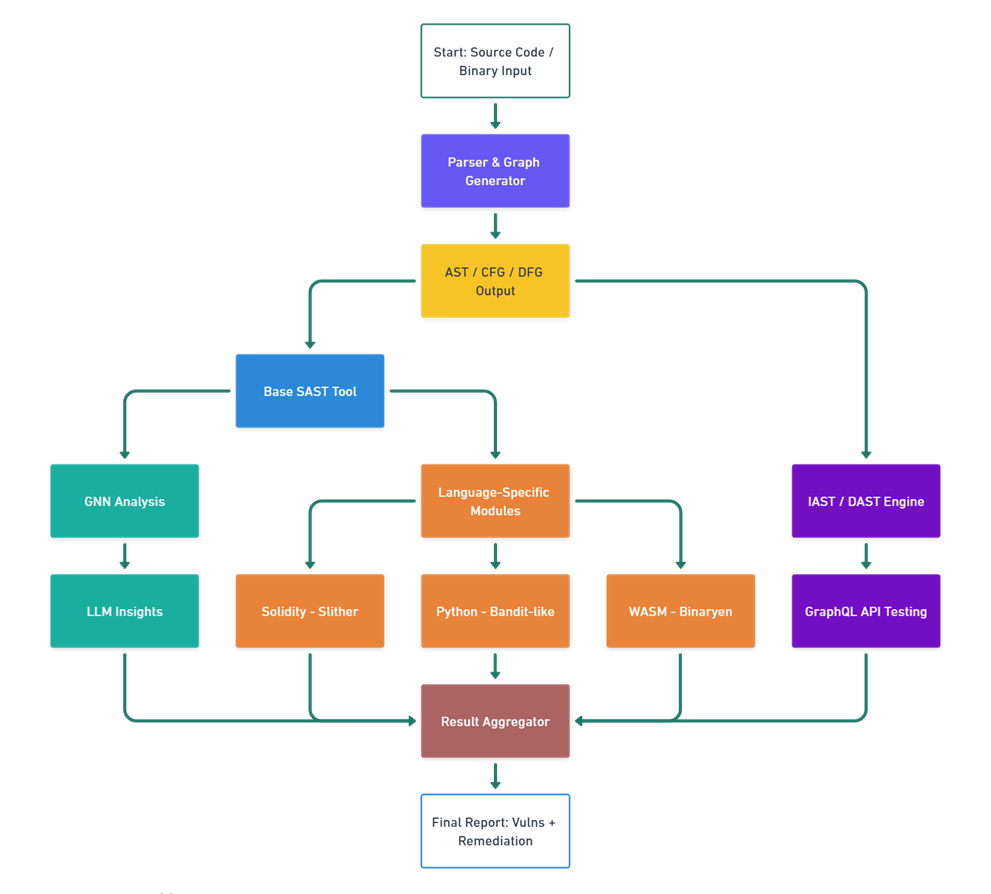
\includegraphics[width=0.6\textwidth]{Figures/overall_flow.png}
\caption{Complete Four-Stage Architecture with Data Flow}
\label{fig:architecture_complete}
\end{figure}

The architecture strategically decomposes vulnerability detection into four stages \textbf{Ingestion \& Parallel Analysis}, \textbf{AI-Powered Filtering}, \textbf{Runtime Confirmation}, and \textbf{Unified Reporting} each progressively filtering false positives while enriching findings with validation evidence. This progressive refinement reduces typical SAST output from 100-500 findings per 10K LOC to 5-15 confirmed vulnerabilities, achieving the target $<$ 15\% false positive rate.

This architecture embodies three design principles: (1) \textit{Progressive confidence building} through multi-stage validation, (2) \textit{Complementary technique integration} combining rule-based, AI-driven, and dynamic approaches, (3) \textit{Intelligent resource allocation} through targeted, uncertainty-driven escalation.

The system's novelty lies in its \textit{Dual-Brain AI analysis} combining Graph Neural Networks (structural code reasoning) with Large Language Models (semantic context understanding), alongside \textit{static-to-dynamic validation} where SAST findings trigger targeted IAST/DAST testing for exploitability confirmation.
}

\section{\uppercase{Stage 1: Ingestion and Parallel Analysis}}

\subsection{Architecture Overview}
\doublespacing{
Stage 1 performs comprehensive static analysis across multiple programming paradigms using five specialized detection engines executing in parallel. This parallel architecture maximizes throughput while maintaining language-specific analysis depth. Table \ref{tab:stage1_modules} summarizes the parallel analysis modules.

\begin{table}[H]
\centering
\caption{Stage 1 Parallel Static Analysis Modules}
\label{tab:stage1_modules}
\footnotesize
\begin{tabularx}{\textwidth}{|l|X|X|}
\hline
\textbf{Module} & \textbf{Target \& Methodology} & \textbf{Key Capabilities} \\
\hline
Base SAST Tool & General-purpose code; Rule-based pattern matching & Insecure API detection, call graph generation, reachability analysis, taint source/sink identification \\
\hline
Python SAST & Python codebases; Bandit-inspired rules & Unsafe library usage (pickle, yaml), insecure functions (eval, exec), Django/Flask-specific vulnerabilities \\
\hline
Solidity SAST & Smart contracts; Slither integration & Reentrancy attacks, integer overflow/underflow, unprotected self-destruct, gas optimization issues \\
\hline
WASM SAST & WebAssembly binaries; Binaryen analysis & Buffer overflows, control-flow hijacking, unsafe memory access, unvalidated imports \\
\hline
Lightweight SAST & Subset of C/similar; Tree-sitter parsing & AST generation, CFG construction, unsafe execution paths, unreachable code detection \\
\hline
\end{tabularx}
\end{table}

\begin{figure}
    \centering
    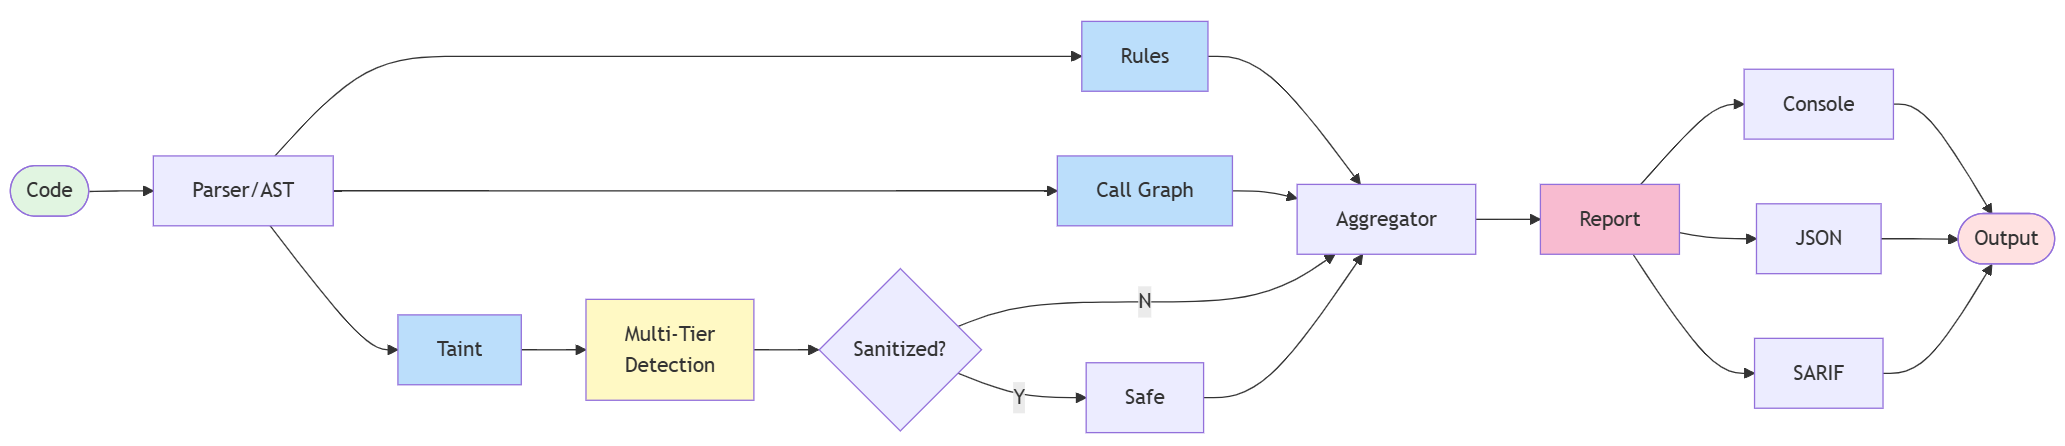
\includegraphics[width=0.95\linewidth]{Figures/stage01.png}
    \caption{Ingestion and Taint Analysis}
    \label{fig:stage01}
\end{figure}

\subsection{Core Components}

\subsubsection{Parser \& Graph Generator}
\doublespacing{
The ingestion layer employs Tree-sitter \cite{tree_sitter} for incremental parsing, generating Abstract Syntax Trees (ASTs) for multiple languages. Tree-sitter's error recovery capability enables analysis of incomplete or syntactically incorrect code  critical for real-time IDE integration. Parsed ASTs feed into graph generators producing Control Flow Graphs (CFGs) and preliminary Data Flow Graphs (DFGs) representing execution paths and data dependencies.

\subsubsection{Base SAST Tool}
\doublespacing{
The Base SAST implements rule-based vulnerability detection through three integrated components:

\textbf{Rule Engine:} Declarative YAML rule specifications defining vulnerability patterns (insecure API calls, dangerous argument patterns, missing security controls). Rules specify pattern matchers (AST node types, function names), severity levels (critical/high/medium/low), CWE mappings, and remediation guidance.

\textbf{Call Graph Analysis:} Constructs directed function call graphs annotated with caller/callee relationships, cyclomatic complexity, and reachability from entry points. Unreachable code vulnerabilities are deprioritized, focusing remediation on executable paths. Edges carry confidence weights: 1.0 for direct intra-file calls, 0.9 for resolved project imports, 0.7 for external libraries, 0.5 for dynamic invocations.

\textbf{Taint Analysis:} Tracks untrusted data flow from sources (user input, file reads, network data) to sinks (SQL execution, command invocation, file writes) without sanitization. This intraprocedural analysis identifies injection vulnerabilities (SQL injection, command injection, path traversal) with high confidence through multi-tier detection: Tier 1 (Exact Match), Tier 2 (Module Classification), Tier 3 (Semantic Object Tracking), Tier 4 (Heuristic Detection).
}


\subsection{Stage 1 Output}
\doublespacing{
Stage 1 produces standardized SARIF 2.1.0 reports containing:

\begin{itemize}
\item Vulnerability findings with CWE mappings, severity (critical/high/medium/low), confidence scores
\item Source locations (file, line, column ranges) with code snippets
\item Taint flow paths (source $\rightarrow$ intermediate steps $\rightarrow$ sink) with sanitization detection
\item Call graph metadata (reachability, cyclomatic complexity, caller count)
\item Preliminary classification: \textbf{Potential} (requires further validation)
\end{itemize}

High-volume findings (typically 100-500 per 10K LOC) escalate to Stage 2 for AI-powered filtering. The output includes both machine-readable SARIF and human-readable console summaries for immediate developer review.
}

\section{\uppercase{Stage 2: AI-Powered Filtering and Enrichment}}

\subsection{Dual-Brain AI Architecture}
\doublespacing{
Stage 2 implements novel \textit{``Dual-Brain'' AI analysis} combining complementary reasoning modes to achieve 60-70\% false positive reduction while maintaining high recall. Figure \ref{fig:dual_brain} illustrates the architecture.

\begin{figure}
    \centering
    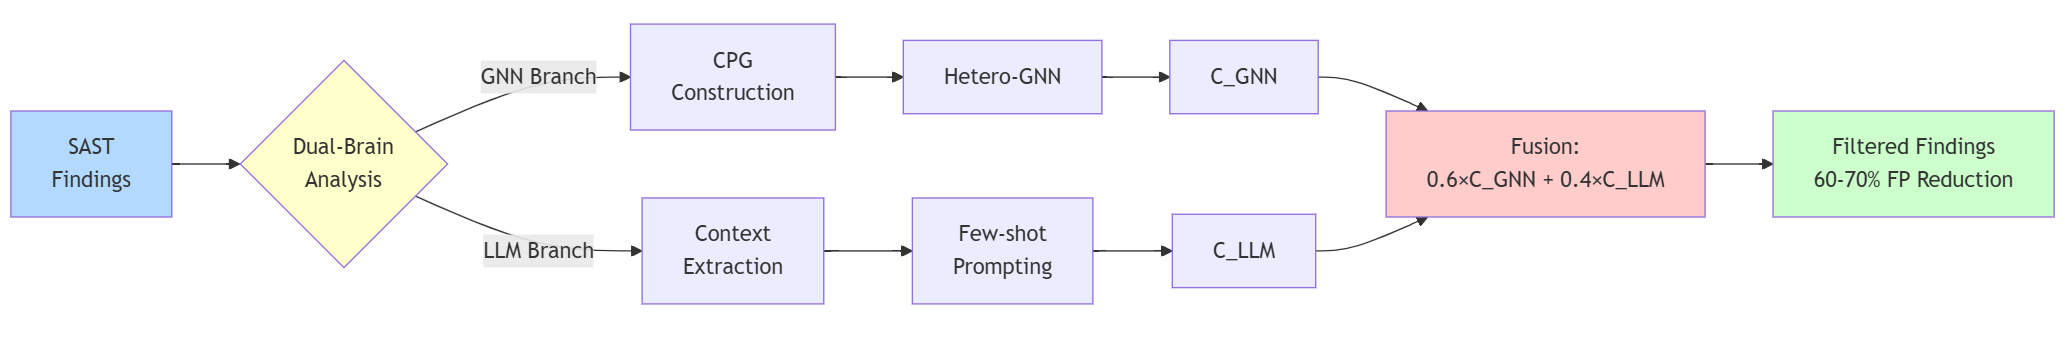
\includegraphics[width=0.95\linewidth]{Figures/stage02.png}
    \caption{Dual-Brain AI: GNN Structural + LLM Semantic Analysis}
    \label{fig:dual_brain}
\end{figure}

\textbf{GNN Brain (Structural Reasoning):} Graph Neural Networks analyze code structure via Code Property Graphs (CPGs) unifying AST, CFG, and DFG representations. Heterogeneous GNN architecture with type-specific message passing detects complex, non-pattern-based vulnerabilities through structural pattern recognition. GNN excels at identifying vulnerability classes requiring graph-level reasoning (e.g., multi-hop taint flows, complex control dependencies).

\textbf{LLM Brain (Semantic Understanding):} Large Language Models (fine-tuned on security-specific corpora) provide contextual semantic validation. LLM analyzes code snippets + SAST findings, determining whether flagged patterns constitute genuine vulnerabilities given surrounding context (e.g., distinguishing sanitized from unsanitized inputs, recognizing framework-provided protections).
}


\subsection{Stage 2 Output}
\doublespacing{
Filtered findings (typically 30-50 per 10K LOC, representing 60-70\% false positive reduction) advance to Stage 3. Each finding carries:

\begin{itemize}
\item Enhanced confidence score (GNN + LLM fusion): 0.5-1.0 range
\item Natural language explanation (LLM-generated, 2-4 sentences)
\item Remediation suggestions (ranked by effectiveness and implementation cost)
\item Classification: \textbf{Likely} (high-confidence, AI-validated)
\item Taint path visualization with CPG node/edge references
\end{itemize}

High-confidence findings ($Confidence_{final} > 0.8$) are prioritized for Stage 3 runtime testing to optimize resource allocation.
}

\section{\uppercase{Stage 3: Runtime Confirmation}}

\subsection{Dynamic Validation Strategy}
\doublespacing{
Stage 3 transitions from static inference to dynamic proof through targeted runtime testing. Rather than exhaustive dynamic analysis (prohibitively expensive),   Multi-Stage Code Security Framework for Adaptive Vulnerability Triage and Detection selectively tests high-priority findings flagged by Stages 1-2, optimizing resource allocation. Figure \ref{fig:dynamic_validation} illustrates the workflow.

\begin{figure}
    \centering
    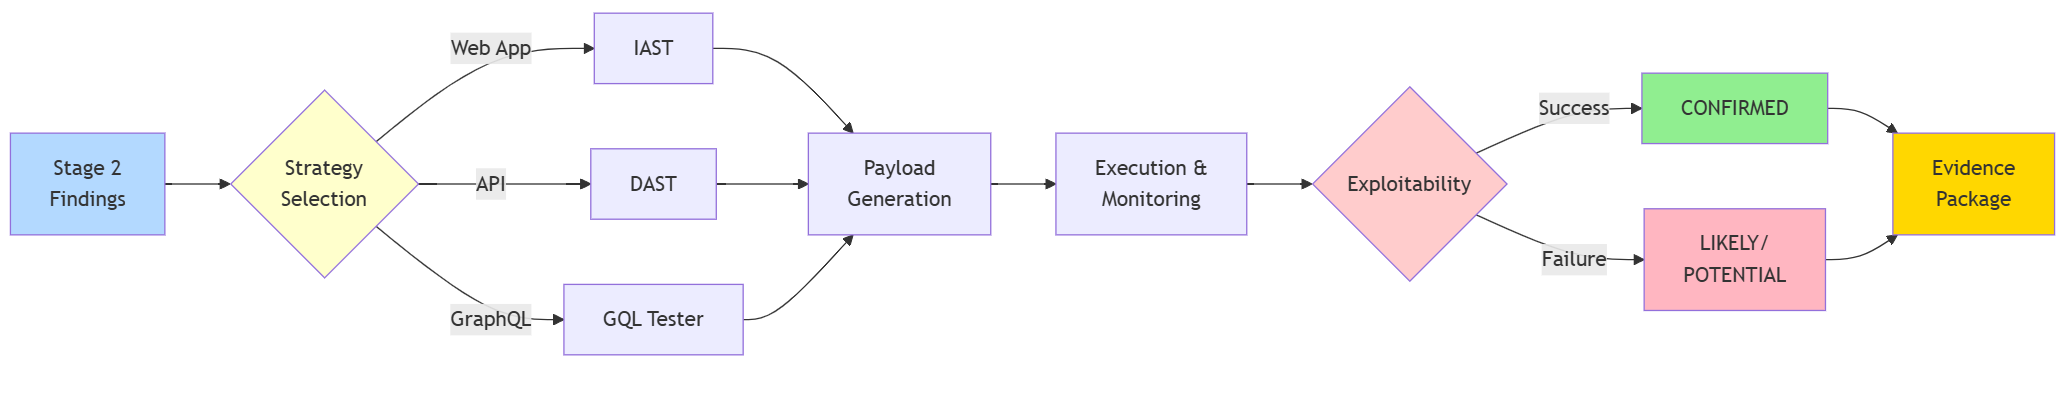
\includegraphics[width=0.9\linewidth]{Figures/stage03.png}
    \caption{Targeted Dynamic Validation Workflow}
    \label{fig:dynamic_validation}
\end{figure}


% \subsection{Interactive Application Security Testing (IAST)}
% \doublespacing{
% IAST instruments target applications at runtime, injecting monitoring hooks that track data flow through actual execution paths.

% \textbf{Instrumentation Architecture:} OpenTelemetry agents inserted at application boundaries and internal propagation points:

% \begin{itemize}
% \item \textbf{Boundaries:} HTTP handlers (Flask/Django routes), database clients (SQLAlchemy, psycopg2), file I/O operations, network sockets
% \item \textbf{Propagation:} Variable assignments, function calls with tainted arguments, object method invocations, string operations (concat, format)
% \end{itemize}

% \textbf{Runtime Taint Validation:} For each SAST-flagged taint flow, IAST verifies whether untrusted data actually reaches dangerous sink during normal application usage. The system maintains a runtime taint map tracking:

% \begin{enumerate}
% \item \textbf{Source tagging:} Mark data from HTTP request parameters, headers, file reads with unique taint identifiers
% \item \textbf{Propagation tracking:} Update taint map as data flows through assignments and transformations
% \item \textbf{Sink detection:} Trigger alert when tainted data reaches SQL query execution, subprocess call, or file write
% \item \textbf{Sanitization recognition:} Clear taint markers when data passes through validated sanitization functions
% \end{enumerate}

% \textbf{Execution Trace Generation:} IAST produces detailed traces including: function call stack, variable values at each step, taint propagation path, and sink invocation parameters. These traces serve as exploitability proof.

% \textbf{Advantage:} White-box approach provides precise exploit confirmation with detailed execution traces (10-20\% performance overhead). However, requires application deployment infrastructure and test environment setup.
% }

% \subsection{Dynamic Application Security Testing (DAST)}
% \doublespacing{
% DAST performs black-box testing by simulating attacker interactions with running applications without requiring source code access or instrumentation.

% \textbf{Attack Simulation Framework:} Selenium/Playwright automates browser interactions, enabling realistic attack scenarios:

% \begin{itemize}
% \item \textbf{SQL Injection:} Submit payloads (\texttt{' OR '1'='1}, \texttt{'; DROP TABLE--}) to form inputs flagged by SAST, observe database errors or authentication bypasses
% \item \textbf{Command Injection:} Inject shell metacharacters (\texttt{; ls -la}, \texttt{| whoami}) into subprocess-invoking parameters
% \item \textbf{Cross-Site Scripting (XSS):} Submit script tags to output contexts, verify execution through DOM inspection
% \item \textbf{Path Traversal:} Test file access with \texttt{../../../etc/passwd} patterns
% \end{itemize}

% \textbf{Exploitability Confirmation:} Successful exploitation indicators include:

% \begin{enumerate}
% \item \textbf{Abnormal responses:} HTTP 500 errors with stack traces, database error messages revealing schema
% \item \textbf{Unauthorized access:} Authentication bypass, privilege escalation to admin accounts
% \item \textbf{Data leakage:} Exposure of sensitive files, database records, or internal system information
% \item \textbf{State modification:} Unexpected database changes, file creation/deletion, or process execution
% \end{enumerate}

% Failed exploits suggest false positives or deployed protections (WAF, input sanitization, parameterized queries).

% \textbf{Advantage:} No source code or instrumentation required; tests deployed application including infrastructure protections. Limited to exercised code paths and requires running application instance.
% }

\subsection{Stage 3 Output}
\doublespacing{
Validated findings (typically 5-15 per 10K LOC, representing definitive vulnerabilities) advance to Stage 4 with:

\begin{itemize}
\item Classification: \textbf{Confirmed} (runtime-proven exploitability)
\item Exploitability proof: IAST execution trace OR DAST attack payload + response screenshot
\item Severity upgrade: Confirmed findings receive severity boost (Medium $\rightarrow$ High, High $\rightarrow$ Critical)
\item Reproduction steps: Detailed instructions for developers to reproduce the exploit
\end{itemize}

Findings that fail exploitation are downgraded to \textbf{Likely} (protected by runtime mitigations) or \textbf{Potential} (possible false positive), preserving developer awareness without false alarm urgency.
}

\section{\uppercase{Stage 4: Unified Reporting}}

\subsection{Evidence Aggregation and Prioritization}
\doublespacing{
Stage 4 synthesizes findings from all stages, applying intelligent prioritization based on multi-source evidence.

\textbf{Three-Tier Classification System:} Table \ref{tab:prioritization} defines the classification criteria.

\begin{table}[H]
\centering
\caption{Three-Tier Vulnerability Prioritization System}
\label{tab:prioritization}
\footnotesize
\begin{tabularx}{\textwidth}{|l|X|X|p{0.18\textwidth}|}
\hline
\textbf{Tier} & \textbf{Criteria} & \textbf{Validation Evidence} & \textbf{Developer Action} \\
\hline
Confirmed & SAST detection + AI validation + Runtime exploitation proof & Stage 1 finding + GNN/LLM confirmation (C $>$ 0.8) + Successful IAST/DAST exploit & Immediate remediation required \\
\hline
Likely & SAST detection + High AI confidence (GNN + LLM agreement) & Stage 1 finding + GNN/LLM confidence $>$ 0.6 + (Not tested OR exploitation failed) & Priority review and remediation \\
\hline
Potential & SAST detection only OR Low AI confidence & Stage 1 finding + (AI confidence $<$ 0.6 OR AI flagged as possible FP) & Manual review recommended \\
\hline
\end{tabularx}
\end{table}

\textbf{Prioritization Formula:} Findings are ranked using multi-factor scoring:

$$Priority = 0.4 \cdot Severity + 0.3 \cdot Confidence + 0.2 \cdot Exploitability + 0.1 \cdot Reachability$$

Where:
\begin{itemize}
\item \textbf{Severity:} Derived from CWE impact rating (Critical=1.0, High=0.75, Medium=0.5, Low=0.25)
\item \textbf{Confidence:} Multi-stage validation score (Confirmed=1.0, Likely=0.7, Potential=0.4)
\item \textbf{Exploitability:} Runtime validation result (Exploited=1.0, Not tested=0.5, Failed=0.2)
\item \textbf{Reachability:} Call graph analysis (Entry point=1.0, Reachable=0.7, Unreachable=0.3)
\end{itemize}

This formula ensures Confirmed vulnerabilities in reachable code with high severity receive top priority, while Potential findings in dead code are deprioritized.
}


  \section{\uppercase{Key Architectural Innovations}}
  \doublespacing{
  \textbf{1. Progressive Refinement:} Four-stage filtering (100-500 → 5-15 findings) addresses alert fatigue.

  \textbf{2. Dual-Brain AI:} Novel GNN-LLM fusion (60/40 weighted) combines structural and semantic reasoning.

  \textbf{3. Static-to-Dynamic Bridge:} Selective testing ($Confidence > 0.8$) reduces testing time by 70-85\%.

  \textbf{4. Modern Technology Support:} Specialized engines for WebAssembly, Solidity, GraphQL.

  \textbf{5. Developer-Centric:} Natural language explanations, code examples, confidence-based prioritization.

  \textbf{6. Heterogeneous CPG:} Unified graph (8 node types, 9 edge types) enables GNN analysis and extensibility.
  }

